\documentclass[12pt]{article}

\usepackage{style}

\usepackage{float}

\usepackage{graphicx,url}

\usepackage[brazil]{babel}   
%\usepackage[latin1]{inputenc}  
\usepackage[utf8]{inputenc}  
% UTF-8 encoding is recommended by ShareLaTex

     
\sloppy

\title{Relatório do problema 04\\ Forte Seguro}

\author{Allan Capistrano de Santana Santos\inst{1} Kevin Cerqueira Gomes\inst{2}}

\address{Engenharia de Computação -- Universidade Estadual de Feira de Santana
  (UEFS)\\
  Caixa Postal 252 e 294 -- 44.036-900 -- Feira de Santana -- BA -- Brasil
  \email{\{allan, kevin\}allan.capistrano3@gmail.com\inst{1} kevingomes.uefs@gmail.com\inst{2}}
}

\begin{document} 

\maketitle

\begin{abstract}
  This report aims to present the proposal received to develop a route computing system for a secure transport company. This document contains the stages of system development, ranging from ideas designed to methods used and results obtained.
\end{abstract}
     
\begin{resumo} 
  Este relatório tem como objetivo apresentar a proposta recebida de desenvolver um sistema de computação de rotas para uma companhia de transporte seguro. Neste documento estão contidas as etapas do desenvolvimento do sistema, que vão desde ideias concebidas aos métodos utilizados e resultados obtidos.
\end{resumo}


\section{Introdução}
Por questões de tempo e eficiência, a empresa Forte Seguro, que é responsável por recolher e transportar para os bancos, o dinheiro das empresas da cidade, solicitou para os alunos do MI Programação um programa que seja capaz de calcular o menor caminho entre o ponto de partida e o local de coleta, e entre o local de coleta e o banco, pois estava cada vez mais difícil fazer esses cálculos de maneira manual em uma hora. Além dos cálculos de menor caminho, na aplicação desenvolvida é possível adicionar novos pontos de coleta, bancos e cruzamentos; adicionar novas ligações entre os pontos citados anteriormente; a remoção desses pontos e ligações; e a alteração dos pontos de partida e chegada.

Para a criação do software, foi utilizado a linguagem Java, que é uma linguagem de programação orientada a objetos (POO), e a IDE NetBeans 8.2. O software criado foi desenvolvido para quais quer plataformas desktop, desde que estas tenham suporte e estejam instalados em seu sistema o JRE (Java Runtime Environment) ou JDK (Java Development Kit). Dessa forma, este relatório tem como objetivo mostrar, a metodologia usada, toda a fundamentação necessária, os resultados obtidos e, pôr fim, a conclusão.

\section{Fundamentação Teórica} \label{sec:firstpage}

Para desenvolver o produto em questão, mostrou-se necessária a aquisição de conhecimentos prévios acerca de alguns padrões de projetos, interface gráfica e sobre determinadas estruturas de dados. Esta seção apresenta de forma breve cada um dos elementos que foram utilizados para alcançar a solução do problema.

\subsection{Padrão MVC ({\itshape Model - View - Controller})}
Modelo-Visão-Controlador (do inglês {\itshape Model-View-Controller}) (figura \ref{fig: diagramaMVC}), é um padrão de arquitetura de software que separa a aplicação em três camadas, a camada de interação com o usuário ({\itshape View}), a de manipulação de dados ({\itshape Model}) e a de controle ({\itshape Controller}).
\begin{figure}[H]
    \centering
    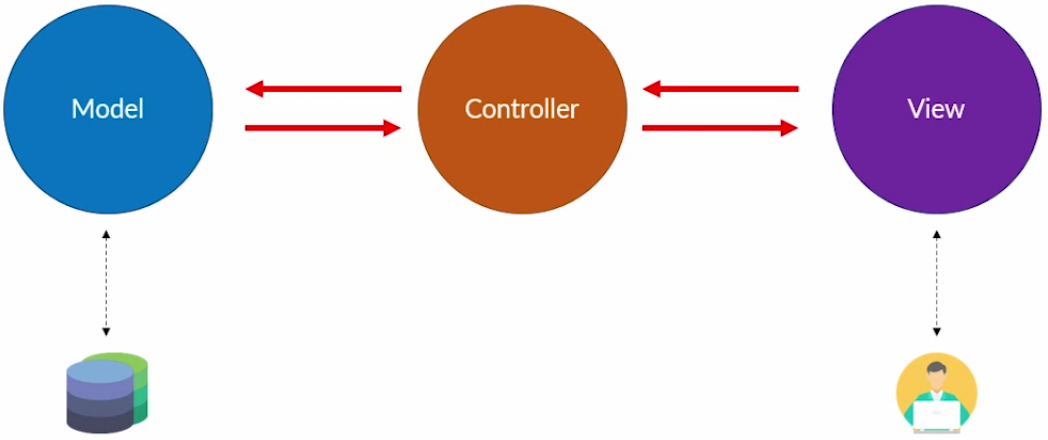
\includegraphics[width=.7\textwidth]{diagrama-do-padrao-mvc.png}
    \caption{Diagrama do padrão MVC \cite{diagramaMVC}}
    \label{fig: diagramaMVC}
\end{figure}

\subsubsection{\itshape{Model}}
O modelo é responsável por tudo que a aplicação irá fazer a partir das instruções do controlador. Em si, ele modela os dados e o comportamento por traz do processo, se atendo apenas com o armazenamento, manipulação e geração de dados.
\subsubsection{\itshape{View}}
A visão ou visualização é a camada de interação do usuário com o programa, em que, é por meio dela que o mesmo pode enviar dados ou comandos que serão passados da {\itshape view} para o {\itshape controller}, e o {\itshape controller} por sua vez fará as devidas alterações solicitadas, na {\itshape model}. Além da entrada de dados, a visão também é a responsável pela exibição dos dados que estão armazenados na {\itshape model}.
\subsubsection{\itshape{Controller}}
O controlador é responsável por receber todas as requisições do usuário, e por controlar todo o fluxo de informações que passa pelo sistema. Seus métodos são os responsáveis por gerenciar os dados que estão localizados na {\itshape model}, definem quais ações são geradas e executadas, para onde essas as informações devem ir e quais dados serão exibidos pela {\itshape view}.

\subsection{Estruturas de Dados}
Para o desenvolvimento do sistema, mostrou-se necessário a utilização de determinadas estruturas de dados, que são organizações de dados e algoritmos que otimizam processos e os deixam mais organizados. Neste caso, foi utilizado para a organização dos dados, a estrutura de dados grafo, que por sua vez utiliza uma outra estrutura em sua composição, o {\itshape ArrayList}.

\subsubsection{Grafo}
Um grafo (Graph) é uma estrutura de dados abstrata formada por um conjunto de vértices e um conjunto de arestas que ligam pares de vértices distintos, e pode ser representado na prática por uma matriz de adjacência, lista de adjacência, mapa de adjacência, lista de vértices e lista de arestas, entre outros. Para o desenvolvimento do programa foi utilizado um grafo ponderado, ou seja, suas arestas possuem um peso, que nesse caso indica o tempo que demora para ir de um poto a outro. E esse grafo foi representado por uma lista de vértices e lista de arestas que se comunicam entre si.

Foi utilizada a estrutura de dados grafo, pois foi dito implicitamente no problema que esta deveria ser a estrutura correta a se utilizar, já que a todo o momento o problema trata sobre pontos, sejam eles de coleta, cruzamento ou banco, e de ligações entre os mesmos. Não sendo necessário dessa forma uma pesquisa a respeito de quais possíveis estruturas de dados se adequariam ao problema em questão.

Como requisito do problema, o software deveria cumprir os testes unitários, seguindo a abordagem Test Driven Development (TDD), que basicamente é uma técnica que se utiliza de testes para verificar se o software está operando de forma correta.

\section{Metodologia}
Devido ao fato do problema ser o primeiro contato com interfaces gráficas para a maioria dos integrantes da turma em questão, os desafios foram acerca do mesmo. Além disso, outro problema pertinente foi sobre o Algorítimo de Dijkstra, ao qual era muito complexo e exigia um pouco mais de atenção.

Como era conhecimento de todos, o problema exigia que usássemos interface gráfica, mas como iriamos fazer? Para essa dúvida, o java oferece duas opções: a biblioteca Swing e a plataforma JavaFX. Os dois são totalmente compatíveis com o problema, e ficou a cargo de cada dupla/pessoa escolher o que usaria. Para nos em questão, optamos pela biblioteca Swing, pois além de ser mais abstrata para nós, tem uma maior facilidade na manipulação de componentes.  

Como requisito do sistema, o software produzido tem que mostrar a menor rota possível entre 3 pontos, e para esse problema, o algorítimo de Dijkstra foi o único conseguiu suprir essa necessidade. Mas a seu desenvolvimento e implementação foi extremamente conturbado, pois se tratava de algo muito complexo para nós. Mas com muita pesquisa e estudo, conseguimos fazer toda a sua implementação e adaptação para o sistema, assim, fazendo com que ele rodasse da forma perfeita para nosso caso.
\section{Resultado e Discussões}

\subsection{{\itshape Model}}
Consiste na base das regras de negócio da aplicação, neste estão contidas as classes responsáveis por armazenar os dados necessários para a execução das operações presentes na classe {\itshape Controller}, e que futuramente serão exibidos na interface gráfica do programa.

\subsubsection{AlgoritmoDijkstra}
A classe AlgoritmoDijkstra tem como única função agrupar os métodos necessários para a execução do algoritmo  concebido pelo cientista da computação holandês Edsger Dijkstra, em que é um algoritmo que calcula o caminho de custo mínimo entre os vértices de um grafo. Primeiramente, é escolhido um vértice como raiz da busca, e então este algoritmo calcula o custo mínimo deste vértice para todos os demais vértices do grafo. Ele é bastante simples e com um bom nível de performance. \cite{algoritmoDijkstra}

Para o desenvolvimento da aplicação, o algoritmo de Dijkstra foi implementado utilizando tipos diferentes de estruturas de dados disponíveis na própria biblioteca {\itshape Collection} do Java. A seguir serão listadas as estruturas utilizadas e suas respectivas funções dentro do programa: 
\begin{description}
\item[•] {\itshape ArrayList}: Foi utilizado para a criação de uma lista que armazenará o resultado da execução do algoritmo, ou seja, nela irá ficarão armazenados os vértices que fazem parte do menor caminho entre um dado par de vértices; 
\item[•] {\itshape HashSet}: Foi utilizado para armazenar os vértices que foram visitados e os que ainda não foram visitados, cada um em um {\itshape HashSet} diferente, o mesmo foi escolhido pois não permitido elementos duplicados, dessa forma não foi necessário fazer um tratamento de exceção, além de sua alta performance no âmbito da busca de elementos; 
\item[•] {\itshape HashMap}: Foi utilizado para armazenar os peso das arestas que compõem o menor caminho entre um par de vértices, e os vértices antecessores, assim como na estrutura citada anteriormente, cada um em um {\itshape HashMap} diferente, o mesmo foi elegido, por conta de seu tempo de busca de elementos ser instantâneo (complexidade O(1)), já que de um elemento adicionado juntamente com uma chave única, por exemplo, o peso de uma determinada aresta é adicionado juntamente a mesma, dessa forma, quando é necessário saber o peso de uma aresta basta buscar pela própria aresta no mapa de pesos, aumentando dessa forma a eficiência do algoritmo e diminuindo o tempo necessário para a execução. E assim como o {\itshape HashSet}, o {\itshape HashSet} não aceita a inserção de elementos repetidos
\end{description}

\subsubsection{Aresta}
A classe Aresta tem como função de armazenar dados a respeito dos vértices que a compõem (vértice de origem e vértice destino) e peso da mesma (grafo ponderado), ou seja, o tempo de deslocamento em minutos entre o vértice de origem e o vértice de destino. E possui métodos para recuperação, modificação e comparação dos dados citados anteriormente.

\subsubsection{Vértice}
A classe Vértice tem como função armazenar dados a respeito dos pontos que serão adicionados no grafo. Os seus atributos são: {\itshape obj} - o identificador do vértice; {\itshape foiVisitado} - utilizado no algoritmo de Dijkstra para verificar se já foi calculada a distância para aquele vértice; {\itshape posX} e {\itshape posY} - coordenadas utilizadas para o posicionamento do vértice na interface gráfica; e {\itshape tipo} - utilizado para identificar o tipo do vértice, ou seja, se é um cruzamento comum, banco, ponto de coleta ou estacionamento. Além de possuir métodos para recuperação, modificação e comparação dos atributos citados anteriormente.

\subsection{{\itshape Controller}}
Consiste na base da comunicação das classes presentes nos pacotes {\itshape view} e {\itshape model}, realizando todas as operações que são requisitadas pelos mesmos para o funcionamento correto e completo do programa.

\subsubsection{Controller}
A classe {\itshape Controller} tem como propósito gerenciar todo o sistema, também como a interface gráfica. Nela, está contido o grafo, além de métodos para a criação do mesmo através do arquivo de texto, inserção de novos vértices, remoção de vértices e arestas, além de métodos para recuperação de dados presentes no grafo e alteração no tipo do vértice (banco, ponto de coleta ou estacionamento).

\subsection{{\itshape View}}
Consiste na base da parte visual do programa, possuindo as classes que compõem a interface gráfica do sistema e de interação do programa diretamente com o usuário.

\subsection{{\itshape Exception}}
Consiste na parte de exceções que o programa pode lançar ao decorrer de sua execução.

\subsubsection{ArestaDuplicadaException}
Exceção relacionada quando o usuário tenta adicionar uma ligação já existente entre dois vértices.

\subsubsection{VerticeDuplicadoException}
Exceção relacionada quando o usuário tenta adicionar um ponto já existente, ou seja, um ponto com um identificador já presente no grafo.

\subsubsection{ArestaNaoEncontradaException}
Exceção relacionada quando o usuário tenta buscar uma aresta que não existe, ou quando o algoritmo de Dijkstra tenta calcular o menor caminho entre dois vértices, porém não existe nenhuma ligação (direta ou indireta) entre os mesmos.

\subsection{{\itshape Test}}
Na pasta e pacote {\itshape test}, estão contidos todos os testes unitários necessários para verificar o completo funcionamento do sistema. A princípio, ocorreram diversos erros e {\itshape warnings}, como: retornos inesperados, exceções de ponteiro nulo e advertências de má prática de uso. Mas por final, todos os problemas foram resolvidos, chegando a 100\% de sucesso de todos os 24 testes unitários, assim cumprindo todas as funções e requisitos do sistema.

\section{Conclusão}
Com o desenvolvimento do programa foi possível adquirir mais conhecimentos a respeito de interface gráfica utilizando o {\itshape Swing} e utilização da estrutura de dados grafo. Tendo seu completo funcionamento testado e comprovado pelos testes unitários, é seguro dizer que o sistema cumpriu todos os requisitos e objetivos propostos, e além dos requisitos propostos, o programa possui uma parte visual do grafo, mostrando os vértices e seus respectivos nomes. O {\itshape software} foi comentado utilizando a ferramenta {\itshape Javadoc} para a documentação das classes e métodos do projeto.

Uma possível melhoria futura seria a exibição das conexões dos vértices, e a exibição do menor caminho modificando a cor das ligações que o compõem.

\bibliographystyle{sbc}
\bibliography{sbc-template.bib}
\end{document}
